\documentclass[12pt,a4paper]{report}

\usepackage[francais]{babel}
\usepackage[utf8]{inputenc}
\usepackage{epigraph}
\usepackage[T1]{fontenc}
\usepackage{listings}
\usepackage{graphicx}
\usepackage{parskip}
\usepackage{xcolor}


%% config
\definecolor{deepblue}{rgb}{0,0,0.5}

\graphicspath{{images/}}
\lstset{
	literate={à}{{\`a}}1,
    language={Python},
    basicstyle=\ttfamily\small, 
    tabsize=4,
    keywordstyle=\bold,
    commentstyle=\color{gray},
    backgroundcolor=\color{lightgray},
    otherkeywords={self},
	keywordstyle=\ttfamily\small\color{deepblue},
    frame=single
    showtabs=false,
    showspaces=false,
    showstringspaces=false
}

\renewcommand{\labelitemi}{∙}
%%macro

\newcommand{\path}[1]{\texttt{#1}}

\newcommand{\codeintext}[1]{\texttt{#1}}

\begin{document}


\title{{\huge Inititation à la programmation}}
\author{Bastien Gorissen \& Thomas Stassin}
\date{Année 2016}

\maketitle
%% \tableofcontents

%\chapter{Level 1}
\begin{figure}[ht]
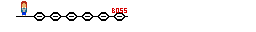
\includegraphics[scale=1]{stage_0.png} 
\end{figure}

\section{Qu’est-ce qu’un langage de programmation?}

\epigraph{Un langage de programmation est une convention pour donner des ordres à un ordinateur. Ce n’est pas censé être obscur, bizarre et plein de pièges subtils.
Ca, ce sont les caractéristiques de la magie.}{\textit{Dave Small}}

Un langage de programmation est un moyen d’intéragir avec l’ordinateur afin de lui donner des instructions, le langage qui est \emph{intelligible}, 
sera \emph{interprété} afin d’être compris par la machine.

\begin{figure}[ht]
\centering
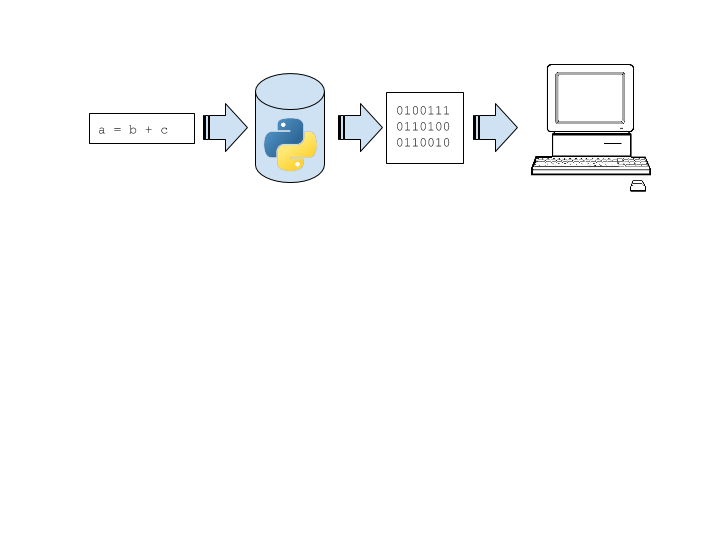
\includegraphics[scale=0.5]{translate_code.png} 
\end{figure}

\subsection{Commentaires}

Si vous ouvrez le script \path{run\_game.py}, vous pourrez voir que certaines lignes commencent par \codeintext{\#}. Celles-ci seront ignorées par l'ordinateur. Ce sont des \emph{commentaires} destinés à clarifier le code.

\subsection{Stage 1-1}
\begin{figure}[ht]
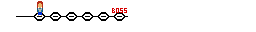
\includegraphics[scale=1]{stage_1.png} 
\end{figure}

Exécuter le script se trouvant dans le dossier \path{lv1/run\_game.py}

\section{Commander à l'ordinateur}

Pour ``commander'' l’ordinateur, on lui donne des \emph{instructions}, le plus souvent, ces instructions seront regroupées dans un \emph{script}.

\subsection{Stage 1-2}
\begin{figure}[ht]
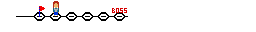
\includegraphics[scale=1]{stage_2.png} 
\end{figure}

Dans l’exercice précédent, nous avons exécuté le script \path{run\_game.py}, ce script est rempli d’instructions, dont celles-ci:

\begin{lstlisting}
    dungeon_size = (5, 5)
    game = world.Game(dungeon_size)
    game.run()
\end{lstlisting}

Que ce passerait-il si on modifiait l’instruction qui définit la grandeur du donjon dans le script ?
Changez les données de dimension du donjon dans le script et observez ce qu'il se passe lors de l'exécution du script.

\subsection{\`{A} retenir}

Python est un \emph{langage sensible à la casse}\footnote{\textit{Case sensitive} en anglais.}, ce qui veut dire qu'il fait la différence entre les majuscules et les minuscules. Autrement dit \codeintext{A} sera différent de \codeintext{a} et \codeintext{world} différent de \codeintext{World}.

Donc si je remplace \codeintext{world} par \codeintext{World} dans le script précédent, il générera une erreur.

\begin{lstlisting}
    dungeon_size = (5, 5)
    game = World.Game(dungeon_size)
    game.run()
\end{lstlisting}

Vous devriez obtenir un message ressemblant à ``\codeintext{NameError: name 'World' is not defined}''

\section{Les instructions de sortie}

Il existe plusieurs sortes d’instructions, l’une d’elles sont les instructions de sortie.
Une instruction de sortie envoie vers une “sortie” ce qu’on lui donne.
Une des sorties les plus couramment utilisée est la console et avec Python, l’instruction de sortie vers la console est \codeintext{print}.

Et donc voici le classique, mais indémodable “Hello World” en Python :

\begin{lstlisting}
    print("Hello World!")
\end{lstlisting}


\subsection{Stage 1-3}
\begin{figure}[ht]
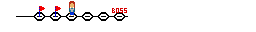
\includegraphics[scale=1]{stage_3.png} 
\end{figure}

Lorsque le donjon est créé, signalez-le par un message dans la \emph{console}.

\section{Les variables}

Souvent, il sera utile de stocker certaines valeurs tout au long de l’exécution de votre code.
Par exemple pour stocker la valeur d’un calcul, ou même afin de réutiliser ses valeurs plusieurs fois. Pour stocker des valeurs, on utilise des \emph{variables}.

La \emph{variable} est un moyen de stocker une valeur quelconque (un nombre, du texte, voire même des \emph{objets} plus complexes) dans la mémoire du programme.

Dans le cas de notre jeu, le donjon, ainsi que le héro sont contenus chacun dans une \emph{variable}.

\begin{lstlisting}
dungeon_size = (5, 5)
game = world.Game(dungeon_size)
hero = Game.hero
\end{lstlisting}

En Python, l’\emph{affectation} d’une valeur se fait avec l’opérateur \emph{=}.

Dans \codeintext{a=3}, on affecte \codeintext{3} à la variable \codeintext{a}\footnote{ En Python il suffit d’affecter une valeur à une variable pour qu’elle commence à exister, ce n’est pas vrai pour la plupart des langages (comme le C\# par exemple).}

\subsection{Stage 1-4}
\begin{figure}[ht]
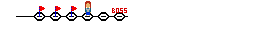
\includegraphics[scale=1]{stage_4.png} 
\end{figure}

Faites en sorte de stocker les dimensions du donjon dans des variables (par exemple \codeintext{length} et \codeintext{width}\footnote{Il est courant d'utiliser des noms de variables en anglais. La programmation est un monde très anglophone.}).

\section{Opérations sur une chaîne de caractères}

Il vous sera parfois utile de savoir manipuler des chaînes de caractères, l'exemple classique est dans une ligne de dialogue, où l'on voudrait dire au héros le nombre d'ennemis qu'il lui reste à tuer avant de finir la quête. Or, lorsque que vous codez, vous ne connaissez pas le nombre d'ennemis. Vous avez sûrement stocké cette information dans une variable et donc vous allez devoir intégrer cette variable à votre ligne de dialogue.

\subsection{Conversion}
Il y un moyen facile de convertir une variable en chaine de caractères\footnote{En Python les chaines de caractères ont le \emph{type} \codeintext{str} pour le mot anglais \textit{string}, qui veut dire chaîne}, il suffit d'utiliser la fonction \codeintext{str}.

Si je voulais convertir la variable \codeintext{nbr\_enemies} qui contient le chiffre \codeintext{3} je procéderais comme suit:

\begin{lstlisting}
	nbr_enemies = 3
	nbr_enemies = str(nbr_enemies)
\end{lstlisting}

A la fin de l'exécution de ce petit script, \codeintext{nbr\_enemies} ne vaut plus \codeintext{3} mais \codeintext{"3"}.

\subsection{Concaténation}
Le fait de coller deux chaînes de caractères l'une derrière l'autre porte un nom: \emph{la concaténation}.
En Python, l'opérateur pour \emph{concaténer} deux variables ensemble est l'opérateur \codeintext{+}.

Par exemple, si je voulais concaténer la variable contenant le nom du héro avec un message cela donnerait :
 
\begin{lstlisting}
	message = ", il te reste des ennemis à tuer."
	message = hero_name + message
\end{lstlisting}

Donc si le héro se nomme Brutor, la chaîne de caractères en fin de script sera égale à \codeintext{"Brutor, il te reste des ennemis à tuer."}

On peut même aller plus loin en mêlant la \emph{conversion} et la \emph{concaténation} en indiquant aussi dans le message le nombre d'ennemis qu'il reste.

\begin{lstlisting}
	message = ", il te reste " + str(nbr_enemies)"
	message = message + " ennemis à tuer."
	message = hero_name + message
\end{lstlisting}

\subsection{Stage 1-5}
\begin{figure}[ht]
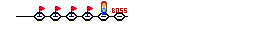
\includegraphics[scale=1]{stage_5.png} 
\end{figure}

Lorsque le donjon est créé, indiquer dans un message à la console la longueur et la largeur de celui-ci.

\section{Les fonctions et les méthodes, première approche}

Pour terminer ce premier level, on va mettre des mots sur deux choses que l'on a vues précédemment. Les \emph{fonctions globales} et les \emph{méthodes}.
Nous avons déjà vu plusieurs fonctions dans les parties précédentes:
\begin{itemize}
	\item[$\bullet$] \codeintext{print}
	\item[$\bullet$] \codeintext{str}
\end{itemize}

Ces fonctions sont dîtes "globales". Ce type de fonctions n'est pas lié à un type d'\emph{objet}.

Il existe aussi une série de fonctions liées à des \emph{objets}, par exemple la fonction \emph{run} de la variable \emph{game}.
On appelle ces fonctions des \emph{méthodes} et elles sont liées à un type d'objets en particulier.

\subsection{Stage 1-6}
\begin{figure}[ht]
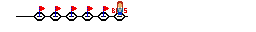
\includegraphics[scale=1]{stage_6.png} 
\end{figure}

La variable du héros, sobrement appelée \codeintext{hero} est du type \codeintext{Hero}, c'est un type de variable que nous avons construit pour le jeu\footnote{Nous verrons plus tard qu'il est possible de définir ses propres types et de leur donner les caractéristiques que l'on désire.}. Nous avons donné trois \emph{méthodes} à cette variable:

\begin{description}
	\item[\codeintext{turn\_left}:] ce qui fait tourner le héros à gauche.
	\item[\codeintext{turn\_right}:] ce qui fait tourner le héros à droite.
	\item[\codeintext{move}:] ce qui fait avancer le héros d'une "case".
\end{description}

Essayez de faire bouger le héros grâce à ces trois méthodes.

\section{Bonus Stage}
\begin{figure}[ht]
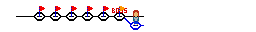
\includegraphics[scale=1]{stage_bonus.png} 
\end{figure}

Pour compléter le stage bonus il faut que vous arriviez à amener le héros sur la sortie du donjon. La sortie est représentée par la case bleue en haut à gauche de la pièce.
Le donjon doit au moins avoir une longueur et une largeur de 7.

%\chapter{Level 2 - Le labyrinthe}

Savoir commander l'ordinateur est une chose, encore faut-il arriver à lui faire faire des choses intelligentes. Heureusement, tous les languages de programmation proposent une série d'outils qui vont permettre de donner des instructions complexes à la machine.

\section{Comparaison n'est pas raison}

L'un des éléments récurrents en programmation est le besoin d'effectuer des comparaisons, et plus globalement d'évaluer si certains \emph{conditions} sont vérifiées ou pas. Le sujet est vaste, mais tout bon programmeur se doit de savoir écrire les bonnes conditions s'il veut que son code se comporte comme il le veut.

\subsection{Les \codeintext{bool}éens}

Outre manipuler des nombres, des chaînes de caractères et autres listes, il y a un autre type de données omniprésent en Python : les \emph{booléens}.

La définition d'une variable booléenne est une valeur qui peut être soit \emph{vraie}, soit \emph{fausse}. En Python, on représente la valeur vraie par \codeintext{True}, et la valeur fausse par \codeintext{False}.

Comme les booléens sont un type de variables comme les autres, vous avez le droit de manipuler \codeintext{True} et \codeintext{False} comme n'impore quelle autre valeur :

\begin{lstlisting}
    a = True
    b = False
    print(a)
    print(b)
\end{lstlisting}

Tout l'intérêt de ce type de variables va résider dans les opérations spécifiques que l'on peut leur appliquer, et qui permettent d'effectuer des choix par rapport à certains éléments du code.

\subsection{Les comparaisons}

Une façon d'obtenir des valeurs booléennes est d'utiliser les opérateurs dit de comparaison. Vous les connaissez probablement pratiquement tous :

\begin{description}
    \item[\codeintext{<} Plus petit que] Teste si la valeur à gauche de \codeintext{<} est plus petite que celle à droite. 
    \item[\codeintext{<=} Plus petit ou égal à] Teste si la valeur à gauche de \codeintext{<=} est plus petite OU égale à celle à droite.
    \item[\codeintext{>} Plus grand que] Teste si la valeur à gauche de \codeintext{>} est plus grande que celle à droite.
    \item[\codeintext{>=} Plus grand ou égal à] Teste si la valeur à gauche de \codeintext{>=} est plus grande OU égale à celle à droite.
    \item[\codeintext{==} Egal à] Teste si la valeur à gauche de \codeintext{==} est égale à celle à droite.
    \item[\codeintext{!=} Différent de] Teste si la valeur à gauche de \codeintext{!=} est différente de celle à droite.
\end{description}

Rien de bien sorcier, et la comparaison renvoie \codeintext{True} si la condition est remplie, et \codeintext{False} sinon.

A noter, l'opérateur ``égal'' (\codeintext{==}) n'est pas simplement \codeintext{=}, puisque \codeintext{=} est déjà ``pris'' par l'affectation d'une variable.

Voici quelques exemples de comparaisons, avec en commentaire la valeur renvoyée :

\begin{lstlisting}
    a = 3
    b = 5
    c = 3

    a > 5     # False
    a < b     # True
    c == a    # True
    a <= b-2  # True
    a != c    # False
    4 >= 1    # False
\end{lstlisting}

Petite astuce : on peut comparer autre chose que des nombres, bien sûr. Python définit un \emph{ordre} sur beaucoup de types d'objets, par exemple les \emph{string}. \codeintext{``message'' <  ``texte''} renverra \codeintext{True}, car l'ordre est ``lexicographique'' pour le texte (plus ou moins équivalent  à l'ordre alphabétique).

On peut évidemment affecter le résultat d'une comparaison à une variable :

\begin{lstlisting}
    a = 3
    b = 5

    condition = a < b
    print(condition)   # Imprime True
\end{lstlisting}

Voyons maintenant ce qu'on peut faire de beau avec ces fameux booléens, avant de voir les applications vraiment pratiques !

\subsection{L'algèbre booléenne pour les nuls}

Les comparaisons et les valeurs booléennes, aussi intéressantes qu'elles soient (et elles le sont dans de nombreux cas), ne révèlent leur vraie puissance que lorsqu'elle sont combinées via une série de règles inventées par Mr Boole\footnote{Véridique, un nom pareil, ça ne s'invente pas.}. On appelle ces règles l'algèbre booléenne.

Ce cours n'a pas pour vocation de faire de vous des pros de la logique, mais vous rencontrerez très souvent les opérations suivantes...

\subsubsection{La négation}

L'opération de négation, consiste simplement à inverser une valeur booléenne. C'est probablement l'opération la plus courante, et en Python, on la note \codeintext{not}.

\begin{lstlisting}
    not True     # == False
    not False    # == True
\end{lstlisting}

\subsubsection{La conjonction (ET)}

L'opération de conjonction, consiste à vérifier si deux conditions sont toutes les deux vraies. Egalement un cas très courant, et notée en Python \codeintext{and}. Son comportement est très similaire à ce dont on pourrait s'attendre :

\begin{lstlisting}
    True and True     # == True
    True and False    # == False
    False and True    # == False
    False and False   # == False
\end{lstlisting}

En résumé, \codeintext{a and b} ne renvoie \codeintext{True} que si et seulement si \codeintext{a} est vrai, ET \codeintext{b} est également vrai. Dans tous les autres cas, le résultat du \codeintext{and} vaut \codeintext{False}.

\subsubsection{La disjonction (OU)}

L'opération de disjonction est un peu le pendant du ET, et représente un OU. C'est-à-dire, on va vérifier si soit la première condition, soit la seconde, soit les deux, sont vraies. En Python, on la note \codeintext{or}. Son comportement est :

\begin{lstlisting}
    True or True     # == True
    True or False    # == True
    False or True    # == True
    False or False   # == False
\end{lstlisting}

En résumé, \codeintext{a or b} renvoie \codeintext{True} que si au moins \codeintext{a} est vrai, OU \codeintext{b} est vrai. Le seul cas où le résultat du \codeintext{or} vaut \codeintext{False} est si les deux conditions sont fausses.

\subsubsection{L'utilité de tout ça...}

Avec ces quelques règles, qui finalement sont assez logiques, on est capable de réaliser des opérations très complexes, qui vont nous permettre de résoudre énormément de cas. Par exemple, on pourrait écrire une condition du style : ``Le héros à moins de la moitié de ses points de vie et il n'a pas de potion, ou il a un allié qui est en train de le soigner.''

Bien entendu en code ça sera un tout petit peu différent visuellement, mais le principe est là.

Mettons en pratique tout ceci...

\section{Prendre des décisions}

Nous voilà enfin arrivé dans le vif du sujet. Pour que le code écrit par un programmeur soit réactif par rapport aux actions de l'utilisateur, ou même qu'il puisse traiter des cas demandant des réponses différentes, il existe un outil véritablement omniprésent dans tous les languages : les instructions de \emph{contrôle de flux}, plus communément appellées par leur petit nom : \codeintext{if}.

\subsection{\codeintext{if}, version simple}

\codeintext{if} en anglais, se traduit par ``si''. De là, on peut deviner le but de cette instruction : faire quelque chose \emph{si} une condition est remplie.

Et c'est exactement ce qu'il se passe.

Voyons un exemple élémentaire :

\begin{lstlisting}
    a = 3
    if a < 10:
        print(str(a) + " est plus petit que 10 !")
\end{lstlisting}

A votre avis, que se passe-t-il si on change la première ligne par \codeintext{a = 245} ?

Il ne se passe rien. De façon un peu plus précise, l'instruction \codeintext{if} est une instruction de branchement. Si la condition indiquée entre le \codeintext{if} et le \codeintext{:} est remplie (et donc égale à \codeintext{True}), le code indenté\footnote{Nous allons y revenir tout de suite.} qui suit est exécuté, et seulement dans ce cas là.

Comme le \codeintext{if} demande une condition, et donc une valeur booléenne, nous pouvons mettre en pratique ce que nous avons vu dans les sections précédentes.

\begin{lstlisting}
    a = 3
    b = 5
    if a < 10 and b > 3:
        print("Conditions remplies !")
\end{lstlisting}

Qu'est-ce qu'il se passe si \codeintext{b} vaut 2 ? Si \codeintext{a} vaut 12 ?

Et qu'en est-il de cet exemple encore plus compliqué ?

\begin{lstlisting}
    a = 3
    b = 5
    if (a < 10 and b > 3) or (a >= b):
        print("Conditions remplies !")
\end{lstlisting}

Quid si \codeintext{b} vaut -12 et \codeintext{a} vaut 42512 ?

On voit donc que rapidement, l'utilisation de quelques opérations de comparaison et d'algèbre de Boole permettent de définir des cas déjà assez complexes. Mais on peut encore faire mieux ! Avant de voir ça, cependant, passons quelques minutes à parler d'un sujet important, particulièrement en Python.

\subsection{De l'importance de l'indentation}

L'indentation, ou alignement du code, est capital en Python. En effet, à la différence de la plupart des langages, Python n'utilise pas d'accolades pour délimiter les différents blocs de code. A la place, l'indentation va jouer le rôle de différenciateur.

Pour comprendre, voici un petit script :

\begin{lstlisting}
    a = 3
    if a > 10:
        print("Conditions remplies !")
        print("a est plus grand que 10 !")
    print("a vaut " + str(a))
\end{lstlisting}

Les lignes 3 et 4, qui sont alignées, mais un niveau en plus que le reste des lignes, représente un bloc de code séparé. Si vous lancez le script tel quel, seule la dernière ligne sera imprimée à l'écran. Si vous changez le \codeintext{a} pour qu'il vaille 15, le bloc qui suit le \codeintext{if} sera bien exécuté.

Les problèmes d'indentation sont véritablement une source d'erreur courante. Il faut donc vraiment y payer une attention toute particulière.

\subsection{\codeintext{if}, version \emph{full options}}

Quand on utilise un \emph{si}, on a naturellement envie d'utiliser un \emph{sinon}. Ca tombe bien, Python, comme beaucoup de langages de programmation, vous offre cette possibilité. Pour reprendre un exemple vu plus haut et l'étoffer un petit peu :

\begin{lstlisting}
    a = 3
    b = 5
    if a < 10 and b > 3:
        print("Conditions remplies !")
    else:
        print("Les conditions ne sont pas remplies !")
\end{lstlisting}

Le \codeintext{else} dans l'exemple ci-dessus représente le \emph{sinon}. Il indique que le bloc de code qui le suit directement doit être exécuté si et seulement si la condition du \codeintext{if} n'est pas remplie.

Notez qu'il s'agit ici d'un choix exclusif : les deux blocs de code ne peuvent en aucun cas être tous les deux exécutés. Soit la condition du \codeintext{if} est remplie, soit elle ne l'est pas, mais on ne peut pas avoir les deux en même temps.

Dans certains cas, vous aurez plus d'un cas à tester. Python offre une dernière option pour effectuer ça, \codeintext{elif} :

\begin{lstlisting}
    a = 4
    if a < 3:
        print("Condition 1 remplie !")
    elif a < 5:
        print("Condition 2 remplie !")
    elif a < 7:
        print("Condition 3 remplie !")
    else:
        print("Les conditions ne sont pas remplies !")
\end{lstlisting}

Python va évaluer les différentes conditions indiquées dans le \codeintext{if} et \codeintext{elif} les unes après les autres, et exécuter le premier bloc de code pour lequel la condition est vérifiée. Et uniquement celui-là ! Même si les conditions suivantes sont remplies, après avoir exécuter le premier bloc, Python va passer le reste de l'instruction.

Le \codeintext{else} ne sera exécuté que si toutes les conditions sont \codeintext{False}, et uniquement ce cas-là.

Voilà de quoi déjà faire pas mal de choses un peu plus intéressantes. Une fois la notion de choix bien en place, nous pouvons passer à la suite, et apprendre à faire des boucles...

\section{La boucle \texttt{for}, premier acte}

S'il y a bien une chose pour laquelle les ordinateurs sont doués, c'est la répétitions. Contrairement aux humains, un ordinateur ne se fatigue pas, ni ne se lasse des tâches répétitives. Au contraire, la possibilité d'effectuer rapidement des opérations similaires sur un grand nombre d'objets ou de données constitue l'une des plus grande force de l'informatique.

D'ailleurs, au coeur de tout jeu vidéo, on trouve une boucle. En simplifiant, l'ordinateur est pris dans un cycle comme suit :

% T: je pense que lstlisting risque de pas affiché les accentuée (il faut donc ajouter dans le "literate" de lstset (cours.tex) pour obtenir les bons accentués. 
\begin{lstlisting}
    Tant que le joueur ne quitte pas le jeu:
        Vérifier si un bouton a été pressé
            Si oui, calculer la réaction
        Afficher le jeu mis à jour
        Recommencer
\end{lstlisting}

Les boucles sont donc un élément extrêmement important dans la boite à outils d'un programmeur. Mais avant d'écrire notre première boucle, faisons un petit détour pour apprendre un élément qui nous aidera.

\subsection{\texttt{range()} ou comment générer une séquence}

Python propose une série de fonctions permettant de gagner un temps précieux dans l'exécution de tâches courantes. L'une des plus courante est \texttt{range()}, qui permet de générer une série de nombres entiers.

La façon la plus simple de l'utiliser est simplement :

\begin{lstlisting}
    range(10)
\end{lstlisting}

Ce qui génère la série suivante :

\begin{lstlisting}
    [0, 1, 2, 3, 4, 5, 6, 7, 8, 9]
\end{lstlisting}

Ou, en généralisant, si \texttt{N} est un nombre entier :

\begin{lstlisting}
    range(N)
\end{lstlisting}

Le code renverra la série suivante :

\begin{lstlisting}
    [0, 1, 2, ... , N-1]
\end{lstlisting}

Le \texttt{N-1} est important ! La liste contient bien \texttt{N} éléments, mais ceux-ci commencent à \texttt{0}, et s'arrêtent à \texttt{N-1}. C'est une subtilité, mais à laquelle on s'habitue assez vite. En informatique, on commence souvent à compter à partir de 0 et non de 1.

Pour visualiser le résultat de \texttt{range()}, on peut utiliser la fonction \texttt{list()} qui crééera une liste intelligible pour nous à partir de la séquence renvoyée par \texttt{range()}. Mais un exemple vaut mieux qu'un long discours :

\begin{lstlisting}
    my_sequence = range(10)
    my_list = list(my_sequence)
    print(my_sequence)
\end{lstlisting}

A propos, on peut enchaîner les commandes pour condenser un peu le code :

\begin{lstlisting}
    print(list(range(10)))
\end{lstlisting}

Mais attention à ne pas se perdre dans les parenthèses !

Avant de voir comment utiliser \texttt{range()} pour contrôler une boucle, voyons encore rapidement 2 autres éléments.

Il est possible de générer une séquence qui va de \texttt{A} à \texttt{N-1} en écrivant

\begin{lstlisting}
    range(A, N)
\end{lstlisting}

Et si on voulait générer une séquence qui progresse par pas de 5 par exemple ?

\begin{lstlisting}
    range(0, N, 5)
\end{lstlisting}

Pour résumer:

\begin{lstlisting}
    range(start, end, step)
\end{lstlisting}

Où \texttt{start} est le point de départ de la séquence, \texttt{end} la fin de la séquence +1, et \texttt{step} l'incrément entre deux éléments de la séquence.

Bonus : comment faire une séquence qui compte de 10 à 1 ? Une idée ?

\subsection{Le réveil de la \texttt{for}(ce)}

Passons sur le titre grammaticalement incorrect de cette section, et intéressons-nous au véritable sujet qui nous intéresse : Comment créer une boucle en Python ?

Il existe plusieurs instructions de boucle en Python, la première que nous allons voir est une boucle dite \emph{arithémtique}, aussi appellée boucle \texttt{for}. 

La boucle \codeintext{for} va parcourir une \emph{séquence} d'éléments, comme une liste ou un tuple, et va effectuer le code qu'elle contient pour chaque élément de la séquence. Un exemple vaut mieux qu'un long discours :

\begin{lstlisting}
    for i in range(10):
        print('Compteur : ' + str(i))
\end{lstlisting}

Le résultat sera l'impression dans la console des nombres de 0 à 9 (souvenez-vous, Python commence à compter à 0, et va jusqu'au nombre qu'on lui a donné, -1).

Et c'est l'entierté de ce qu'il faut savoir pour utiliser une boucle \codeintext{for} ! Comme le montre l'exemple, la boucle est dirigée par une variable spéciale, ici \codeintext{i}, qui est appelée ``compteur''. On peut l'utiliser, à l'intérieur de la boucle, comme une variable normale.

Il existe un autre type de boucle, sans compteur, mais nous en parlerons plus tard dans le cours.

% Level 3:
% Matière:
% ● Boucle logique (while)
% ● Comprendre l’utilité des fonction (et des méthodes)
% ● import de \emph{module} Python
% ● utilisation de nombres aléatoires
% Exercices:
% 1. Remplacer la boucle for du bonus stage du level 2 par une boucle while
% conditioner sur la victoire (arrivée à la fin du labyrinthe) du héro.
% 2. Coder le mouvement des ennemis pour qu’il bouge de manière aléatoire, tout en
% évitant les obstacles.
% Bonus Stage:
% Faire sortir le héro du du donjon en évitant les obstacles et en attendant que les
% ennemis

% horaire du cours:

% 8h45
% 10h30
% 12h15
% 13h15
% 15h00
% 16h45


% présence: 10 min.
% -- 8h55
% Révision:
% 	Exercice: 30 min.
%	Correction: 20 min.  
% -- 9h45
% Boucle while 5 min.
% Exercice 10 min.
% -- 10h00
% Import module personnelle 5 min + Exercice : 5 min.
% Import module Python: 5 min.
% Excercice Random : 5 min.
% -- 10h15
% Explication du random: 5 min
% Exercices sur le random: 10 min
% PAUSE

\chapter{Level 3}

\section{Les boucles logiques}

On a vu dans le chapitre précédent, la boucle dîtes arithmétique. Avec cette boucle, la partie de code \emph{contrôlée} par celle-ci, s'exécute un nombre de fois précis.

Parfois, on sera intéressé que le programme s'arrête, non pas après un certain nombre de fois, mais plutôt lorsque qu'une certaine condition est remplie. Pour se faire on fait appelle au \emph{boucle logique}.

En python, c'est l'instruction \codeintext{while}\footnote{"Tant que" en anglais} qui est utilisée.

Cette instruction doit être suivit d'une \emph{condition}, celle-ci va déterminé à chaque \emph{itération}, si le programme doit continuer ou non d'exécuter la boucle.

Dans le script suivant, la boucle sera exécuter tant qu'il reste des monstres.

\begin{lstlisting}
while monsters_nbr >= 0:
	hero_kills = hero.attacks()
	monster_nbr = monster_nbr - hero_kills
	game.run()
\end{lstlisting}

La méthode \codeintext{attacks} de la variable \codeintext{hero} renvoie 1 ou 0, donc il est impossible de savoir combien d'itération seront nécessaire pour réduire la variable \codeintext{monsters\_nbr} à 0.
C'est donc un \emph{boucle logique} qui utilisée dans ce genre de cas.

%% voir dans le level 2 comment Bastien parle  des booleens.
La condition qui contrôle la boucle est similaire à la condition utilisée avec l'instruction \codeintext{if}.
La boucle s'arrête lorsque la condition est \emph{faux}.

Dans le cas de notre script, c'est lorsque le nombre de monstre passe en-dessus de 0 que la condition devient \emph{fausse}.

\subsection{\`A retenir}

\textbf{Très, très, très important}: il est impératif quà l'intérieur de votre \emph{boucle logique}, il y ait un moyen de rendre la condition de contination fausse. Sinon vous allez vous retrouver face à une boucle infinie. 

\subsection{Stage 3-1}

Reprenez le \textit{bonus stage} du \textit{level 2}\footnote{au besoin le code corrigé de cette exercices ce trouve dans le script \path{bonus\_stage\_2.py}}. Arrangez ce code avec une \emph{boucle logique} à la place de la \emph{boucle arithmétique} pour le héros arrête de bouger dès qu'il est arrivé à destination et non après un nombre d'itération arbitraire.
Lorsque le héros a atteint sa cible, la variable \codeintext{hero.is\_at\_goal} vaut \codeintext{True}, dans les autres cas elle est égale à \codeintext{False}.

\section{imports}

En Python, il est courant de devoir \emph{importer} le contenu de fichier dans d'autre fichier.
\`A plusieurs reprise, on déjà vu cette instruction dans les scripts que l'on a utilisé:

\begin{lstlisting}
import world
\end{lstlisting}

Cette commande, demande à python d'\emph{importer} le contenu du fichier \path{world.py} en vue de l'utiliser plus tard.
Dans la suite, si l'on veut faire appel au contenu de \codeintext{world}, on doit utilisé son nom suivit d'un "\codeintext{.}"

Par exemple si je veux utiliser la variable \codeintext{GROUND\_IMAGE\_PATH} dans mon script je vais procéder comme suit:

\begin{lstlisting}
import world

scree_size = world.GROUND_IMAGE_PATH
\end{lstlisting}

On peut aussi n'\emph{importer} qu'une partie d'un \emph{module}\footnote{C'est le nom que l'on donne au fichier que l'on importe}.

\begin{lstlisting}
from world import GROUND_IMAGE_PATH
\end{lstlisting}

En procédant de cette manière, on n'\emph{importe} que la variable \codeintext{GROUND\_IMAGE\_PATH}.
Cela présente l'avantage de ne devoir précédé la variable \codeintext{GROUND\_IMAGE\_PATH} de \codeintext{world.}, on peut se contenter du nom de la variable seul.

\begin{lstlisting}
from world import GROUND_IMAGE_PATH

screen_size = GROUND_IMAGE_PATH
\end{lstlisting}

Et enfin, on peut \emph{importer} plusieurs composant d'un \emph{module} sur la même ligne.
Si je voulais importer \codeintext{GROUND\_IMAGE\_PATH} et la variable \codeintext{OBSTACLE\_IMAGE\_PATH}, je procéderais ainsi:

\begin{lstlisting}
from world import GROUND_IMAGE_PATH, OBSTACLE_IMAGE_PATH
\end{lstlisting}

\subsection{Stage 3-2}
Dans le fichier \path{data.py}, se trouve toute les données utilisées pour le jeu. Parmis c'est données se trouve la donnée de la \textit{taille de la fenêtre du jeu} : \codeintext{SCREEN\_SIZE} (c'est un \codeintext{tuple} correspondant à \codeintext{(\textit{largeur},\textit{hauteur})} et la donnée du \textit{facteur de grossissement}: \codeintext{SCALE\_FACTOR}.
La grandeur réelle de l'écran est calculée en multipliant la \textit{largeur} et la \textit{hauteur} de l'écran par le \textit{facteur de grossissement}.
\emph{Importer} ces données dans le \codeintext{run\_game} et affichez dans la console la taille réelle de la fenêtre de jeu.

\subsection{N'Import quoi!}

Il n'y a pas que les \emph{modules} que vous avez fait que vous pouvez \emph{importer}, Python est livré avec un série \emph{module} prêt a être utilisé par vos mains avides de coder.
Pour importer ces \emph{modules}, il n'y a pas de différences que pour vos \emph{modules} personnelles. il suffit juste de connaitre le nom du \emph{module} que vous voulez importer\footnote{La liste des modules disponibles dans Python est leur contenu est disponible sur le site de Python (\url{www.python.org/doc})}. L'un de ses modules qui nous sera très utiles dans le cadre de la réalisation de jeu vidéo, c'est \codeintext{random}.

Pour l'importer donc pas de mystère:

\begin{lstlisting}
import random
\end{lstlisting}

\subsection{Stage 3-3}
Ce module contient la fonction \codeintext{(randint)} cette fonction prend deux arguments qui doivent être de type \codeintext{int}.
En important cette fonction et uniquement cette fonction (Rappelez-vous, les méthodes d'\emph{import} de \emph{modules} Python ne sont pas différentes de l'\emph{import} de modules personels), essayez de déterminez que fait la fonction (même si le nom du \emph{module} et de la fonction sont de gros indices).
Vous pouvez utilisez le script \codeintext{run\_game}, ou bien la console Python pour faire ces tests.

\section{La génération de nombre aléatoire}

Vous avez put le constatez, la fonction \codeintext{randint} génère des nombres aléatoires compris entre le premier arguments de la fonction et le deuxième argument\footnote{Pour autant que les arguments soit en ordre croissant, sinon çà génère une erreur.}
Générer des nombres aléatoires est extrêment partique, car cela permet de simuler le caractère hasardeux d'une situation, un peu à l'image d'une dès.

\subsection{Stage 3-4}

Utiliser la fonction random sur le jeu.
Simulez un dé à 6 faces:
\begin{description}
	\item[1]: le héros tourne à droite
	\item[2]: le héros toure à gauche
	\item[3-5]: le héros avance
	\item[6]: le jeu héro arrête de bouger définitivement
\end{description}

En plus de cela, à chaque lancer de dé: affichez dans la console le résultat de celui-ci.



\end{document}